\documentclass[12pt,titlepage, a4paper, oneside, openright, listof=totoc, headings=normal, chapterprefix=true]{scrbook}

\addtokomafont{disposition}{\rmfamily}
% FIGURES %

\usepackage{palatino} % Type of font

%\usepackage{fancyhdr} % Change caption style; changes headers and page styles etc.%
\usepackage[doublespacing]{setspace} % For changing line spacing
\usepackage[UKenglish]{babel}
\usepackage{csquotes} % Quotes

\usepackage{array}
\usepackage{alphalph}
\usepackage{booktabs,longtable,rotating,threeparttable,threeparttablex,multirow,pdflscape}
\usepackage{microtype} % makes pdf look better

\usepackage{eurosym}
\usepackage{amsmath}
\usepackage{amsfonts}
\usepackage{amssymb}
\usepackage{subfig}
\usepackage{eqnarray}
\usepackage{fancyref}
\usepackage[capposition=top]{floatrow} 

	
\usepackage{placeins} 					% Allows the use of \FloatBarrier

\usepackage[left=2.6cm,top=2.5cm,right=2.6cm,bottom=2.5cm, footnotesep=\baselineskip]{geometry}
\usepackage{soul,color}
\usepackage[dvipsnames]{xcolor}
\usepackage[colorlinks = true,
            linkcolor = BrickRed,
            urlcolor  = blue,
            citecolor = black,
            anchorcolor = grey]{hyperref}



\usepackage{graphicx}
\usepackage{epstopdf}
\usepackage{lscape} % Enables turning single pages into landscape mode
\usepackage{adjustbox}
\usepackage[toc, page]{appendix}

\soulregister\citep7
\soulregister\citet7
\soulregister\ref7

\usepackage[
	style=authoryear,
	natbib=true,
	firstinits=true,
       uniquename=false,
       uniquelist=minyear,
       maxcitenames=2, maxbibnames=99,
	backend=biber]{biblatex}
	\addbibresource{bibliography.bib}

% BIBLIOGRAPHY %
\renewbibmacro{in:}{%
  \ifentrytype{article}{}{\printtext{\bibstring{in}\intitlepunct}}}  % remove 'in:' preceding article title
\renewcommand*{\nameyeardelim}{\addspace} % no comma between author and year in-text citations
\DeclareFieldFormat[article]{volume}{#1\addcolon\space}

\DeclareFieldFormat{pages}{#1}% no prefix for the `pages` field in the bibliography
\DeclareFieldFormat{journaltitle}{\mkbibemph{#1},} % italic journal title with comma

% Place volume number within parentheses:
\renewbibmacro*{volume+number+eid}{
 \setunit{Vol.~}
    \printfield{volume}
   \printfield{number}
    \setunit{\addcomma\space}
    \printfield{eid}}
\DeclareFieldFormat[article]{number}{\mkbibparens{#1}}

% Ensure that issue number is not shown if coded in bibliography file
\renewbibmacro*{volume+number+eid}{
\printfield{volume}}

% GENERAL SETTINGS %
\renewcommand{\baselinestretch}{1.5}
\setcounter{secnumdepth}{4} % organisational level that receives a numbers
\setcounter{tocdepth}{3}    % print table of contents for X levels

% Stop footnote counter to be restarted after every chapter.
\usepackage{chngcntr}
\counterwithout{footnote}{chapter}

% Increase space between tables/figures from different chapters in LoF/LoT
\makeatletter
\def\@chapter[#1]#2{\ifnum \c@secnumdepth >\m@ne
                       \if@mainmatter
                         \refstepcounter{chapter}%
                         \typeout{\@chapapp\space\thechapter.}%
                         \addcontentsline{toc}{chapter}%
                                   {\protect\numberline{\thechapter}#1}%
                       \else
                         \addcontentsline{toc}{chapter}{#1}%
                       \fi
                    \else
                      \addcontentsline{toc}{chapter}{#1}%
                    \fi
                    \chaptermark{#1}%
                    \addtocontents{lof}{\protect\addvspace{20\p@}}% NEW
                    \addtocontents{lot}{\protect\addvspace{20\p@}}% NEW
                    \if@twocolumn
                      \@topnewpage[\@makechapterhead{#2}]%
                    \else
                      \@makechapterhead{#2}%
                      \@afterheading
                    \fi}
\makeatother

% Increase space between caption and number/page in LoT/LoF
\makeatletter
\def\l@figure{\@dottedtocline{1}{1.5em}{3em}}
\def\l@table{\@dottedtocline{1}{1.5em}{3em}}
\makeatother

\date{}
\title{}

\begin{document}
\pagenumbering{roman}
\setcounter{page}{1}

\thispagestyle{empty}
\begin{center}
\vspace{1cm}
\normalsize
%\bf
\singlespacing

{\Large\textbf{Essays on the empirical economics}}
\doublespacing
\vspace*{2in} \mbox{} \\
\normalsize %\rm
 Your name here %
\vspace*{1in} \mbox{} \\
Your uni here \\
Your department
\vspace*{0.4in} \mbox{} \\
Date here %
\vspace*{1.4in} \mbox{} 

\small{A thesis submitted to the Department ....\\}
\end{center} 

\newpage

\begin{flushright}
 \textit{Quote here} \\
Whoever said that ...
\end{flushright} % 1) Title	

\addcontentsline{toc}{chapter}{Abstract}
\onehalfspacing	
\chapter*{Abstract}

This is the abstract of the thesis
		% 2) Abstract

\addcontentsline{toc}{chapter}{Table of Contents}
\tableofcontents % 3) Table of contents				
\listoftables 						% 4) List of tables, illustrations, etc
\listoffigures
\clearpage

\addcontentsline{toc}{chapter}{Acknowledgements}%
\chapter*{Acknowledgements}
\renewcommand{\baselinestretch}{1.5}
I am grateful to many people for my helping me to complete the thesis



	% 7) Acknowledgements

\addcontentsline{toc}{chapter}{Declaration}%
%\pagestyle{plain}	
\chapter*{Declaration}
\thispagestyle{plain}

I declare that this thesis is a presentation of original work  
	% 8) Author's declaration
\clearpage

\doublespacing
\pagenumbering{arabic}
\setcounter{page}{1}

\chapter{Introduction}
\label{ch1}


This thesis addresses relevant aspects associated with .....



                 % CHAPTER 1 (Intro)
\singlespacing
\chapter{This is chapter 2}
\label{ch2}
\doublespacing
\chaptermark{Chapter 2: This is.... }

\section{Introduction}
\label{sec: intro}

The chapter 2 consists of .....

\newpage

\begin{landscape}
\section{Figures}
\label{sec: figures}

\begin{figure}[!h]
\centering
  \caption{This is Figure 1}
    \label{fig: maps1}
    
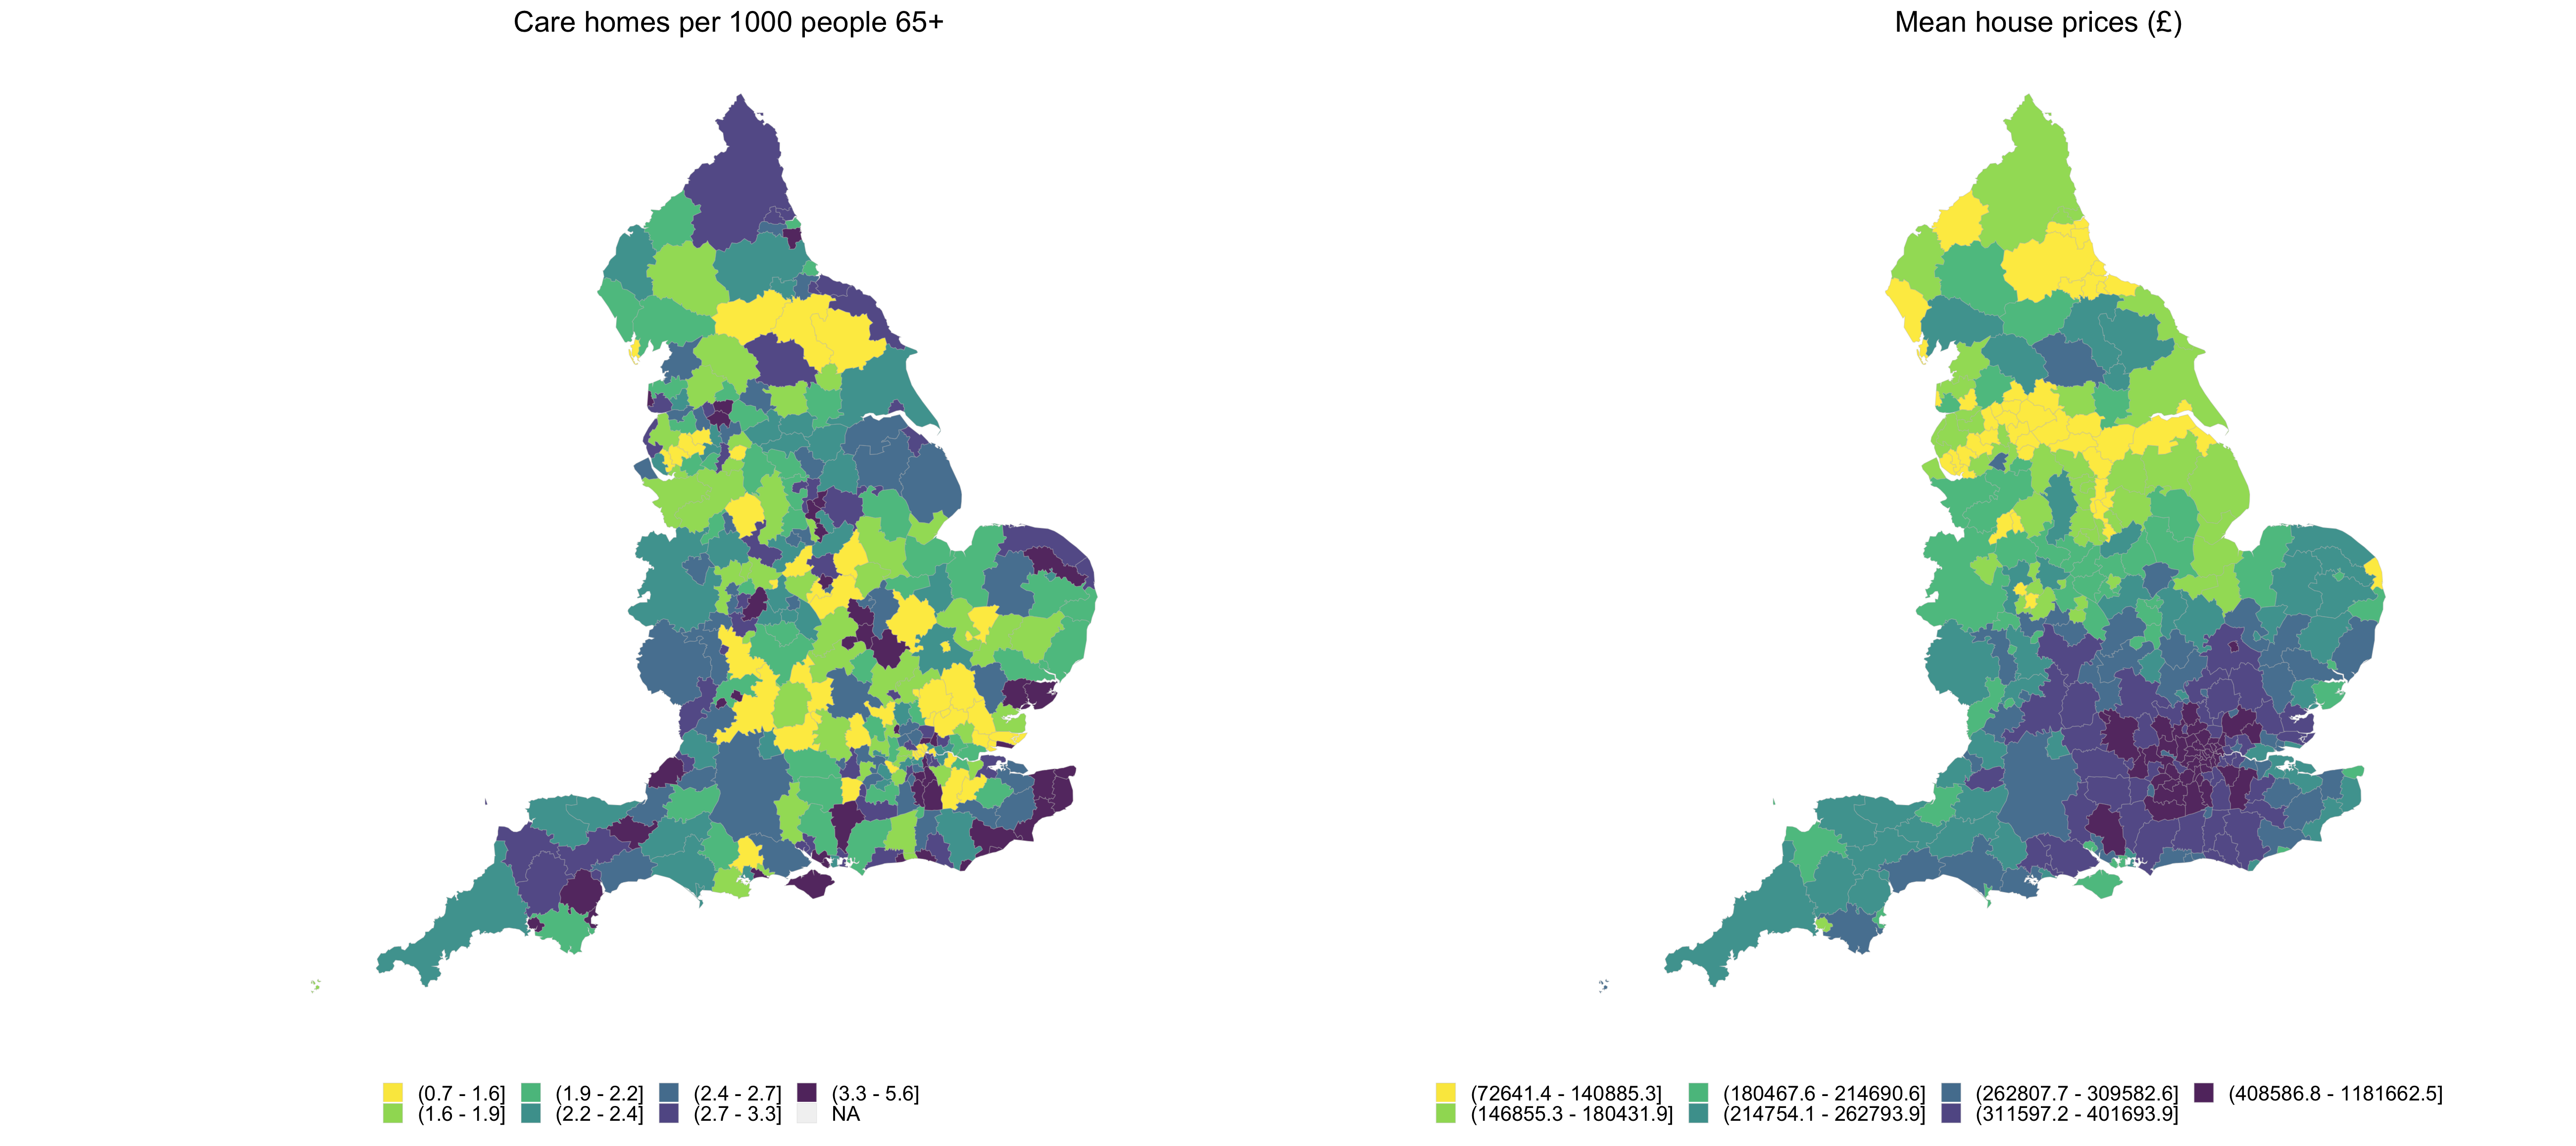
\includegraphics[width=1\textwidth]{ch_2/maps_test.png}


\floatfoot{{\textbf{Note}}: English districts.}
\end{figure}

\end{landscape}

\newpage 

\begin{figure}[!h]
\centering
  \caption{This is figure 2}
    \label{fig: maps2}
    
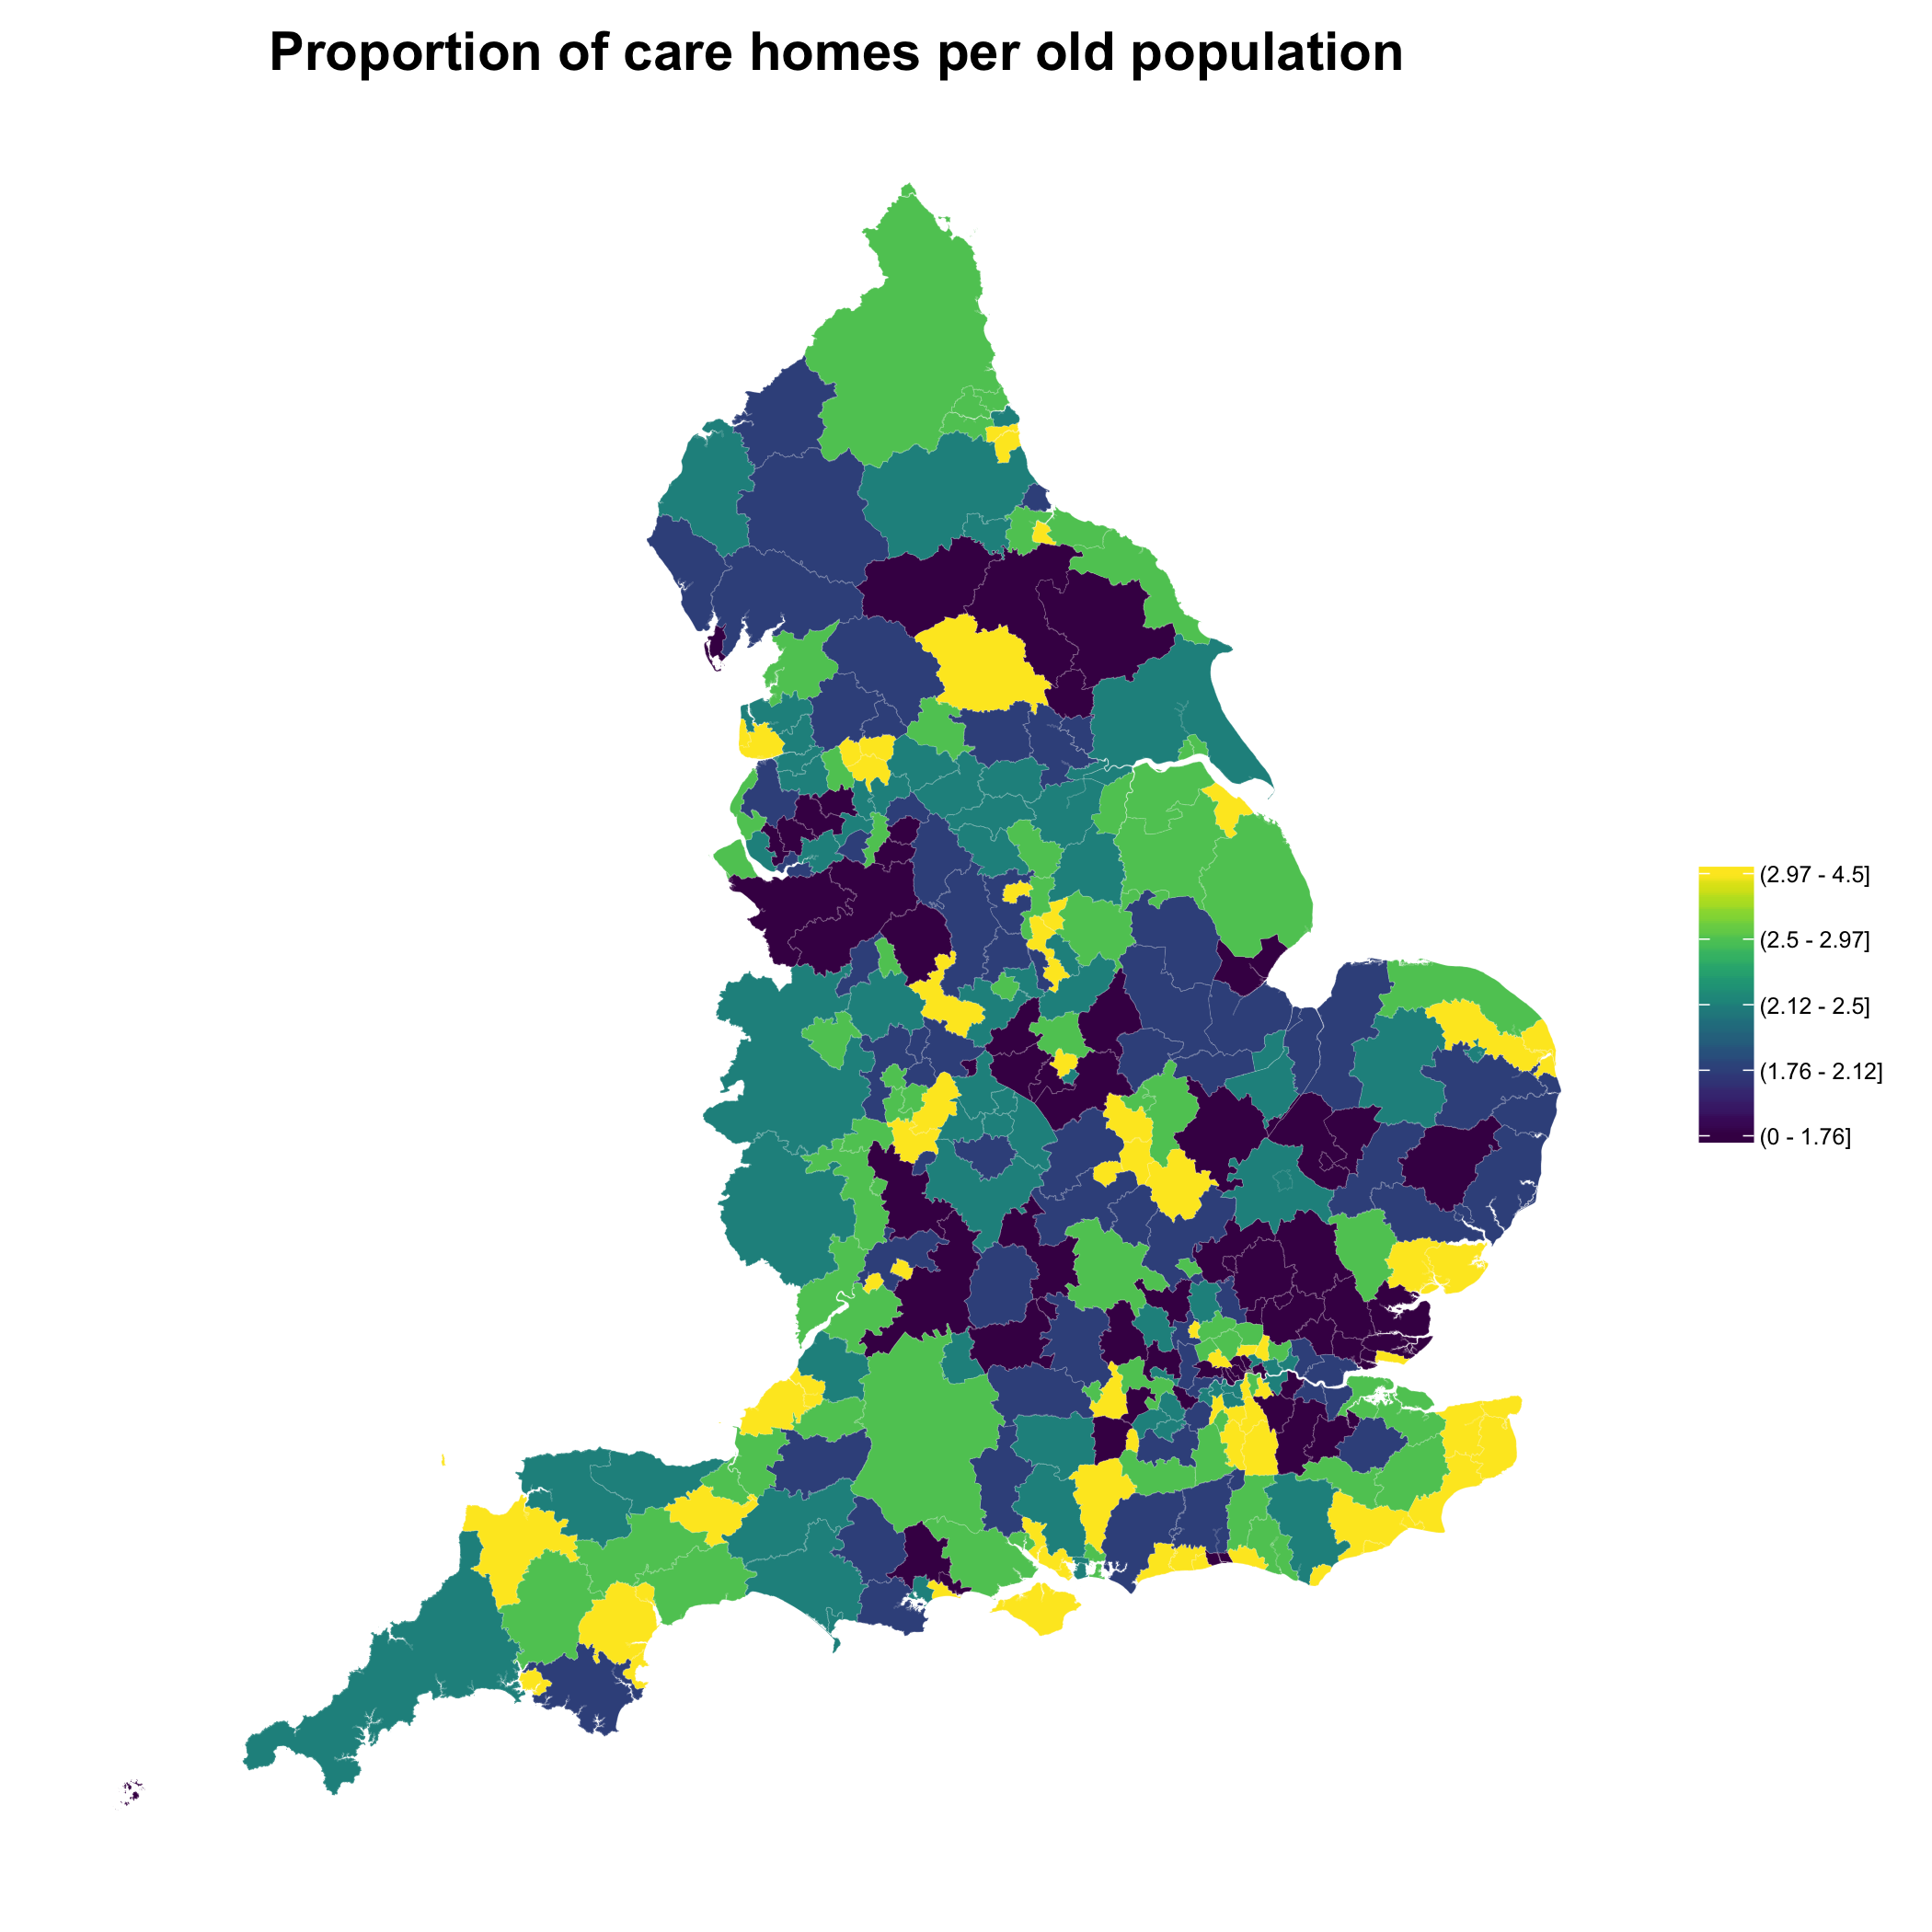
\includegraphics[width=1\textwidth]{ch_2/map_care_homes.png}


\floatfoot{{\textbf{Note}}: Aging}
\end{figure}


\newpage
\section{Tables}
\label{sec: tables}

\begin{table}[!h]
\caption{Your model here}
\label{tab: second_stage}
\resizebox{\textwidth}{!}{%
\begin{tabular}{@{}lccccccc@{}}
\toprule
                           & \multicolumn{3}{c}{Number of care homes per 1000 population 65+} & \multicolumn{1}{l}{} & \multicolumn{3}{c}{Entry rates}   \\ 
                     \cmidrule(r){2-4} \cmidrule(r){6-8} \\
 
                           & (1)                  & (2)                 & (3)                 &                    & (4)       & (5)       & (6)       \\
                          \cmidrule(r){2-4} \cmidrule(r){6-8} \\
Average house prices (log) & -0.780***            & -0.107              & -0.622***           &                      & -0.00385  & -0.0103** & -0.00652  \\
                           & (0.118)              & (0.0898)            & (0.178)             &                      & (0.00478) & (0.00406) & (0.00868) \\
\midrule\\
Estimation                 & OLS                  & IV                  & IV                  &                      & OLS       & IV        & IV        \\
Time FE                    &                      & Yes                 & Yes                 &                      &           & Yes       & Yes       \\
Region FE                  &                      & No                  & Yes                 &                      &           & No        & Yes       \\
\midrule
\\
Observations               & 1260                 & 1260                & 1260                &                      & 1260      & 1260      & 1260      \\
Local Authorities          & 315                  & 315                 & 315                 &                      & 315       & 315       & 315       \\
R-squared                  & 0.209                & 0.043               & 0.204               &                      & 0.021     & 0.014     & 0.048     \\ \bottomrule
\end{tabular}%
}
\begin{tablenotes}
     \scriptsize
      \item  {\textbf{Note}}: Your sources here.  
      Your explanation here . $^{***}p<0.01$,$^{**}p<0.05$, ${^*}p<0.1$ \end{tablenotes}
\end{table}                 % CHAPTER 2
% Add chapters here 
\chapter{Appendices}
\label{appendix}

\section{Appendix to Chapter ....}
\label{sec:label_to_appendix1}
\setcounter{table}{0}
\setcounter{figure}{0}
\renewcommand{\thetable}{A3.\arabic{table}}
\renewcommand{\thefigure}{A3.\arabic{figure}}

This is the appendix ...









 
\addcontentsline{toc}{chapter}{Abbreviations}        
\chapter*{Abbreviations}
%\thispagestyle{plain}

\begin{table}[ht]
\setlength{\extrarowheight}{.4em}
\begin{tabular}{ll}

TFA & This is first abbreviation \\
TSA  & This is second abbreviation \\
TTA & ... \\


\end{tabular}
\end{table}
\printbibliography[heading=bibintoc, title={References}]
									
\end{document}




